First of all, let us examine the different ways by which
antibodies are naturally used by the immune system to combat
a pathogen infection. There are four of them, complementary of each other.

\subsubsection{Antigen neutralization}

\begin{figure}[H]
    \begin{minipage}{0.55\textwidth}
        The most simple way antibodies can act against a pathogen is by
        \emph{neutralization} : the antibodies specific to an epitope of the
        antigen bind to this epitope and form together a complex that surround
        the pathogen \cite{langermans_antimicrobial_1994}.
        It is thus geometrically prevented to act as it normally would 
        by infecting the nearby cells.

        Antibodies acting in this manner are called \emph{neutralizing antibodies}
        or NAbs. The neutralized pathogen cannot approach the cell and
        bind to its surface receptors, thus making it ineffective. 
        The resulting complex can then be eliminated.
    \end{minipage}\hfill
    \begin{minipage}{0.35\textwidth}
        \centering
        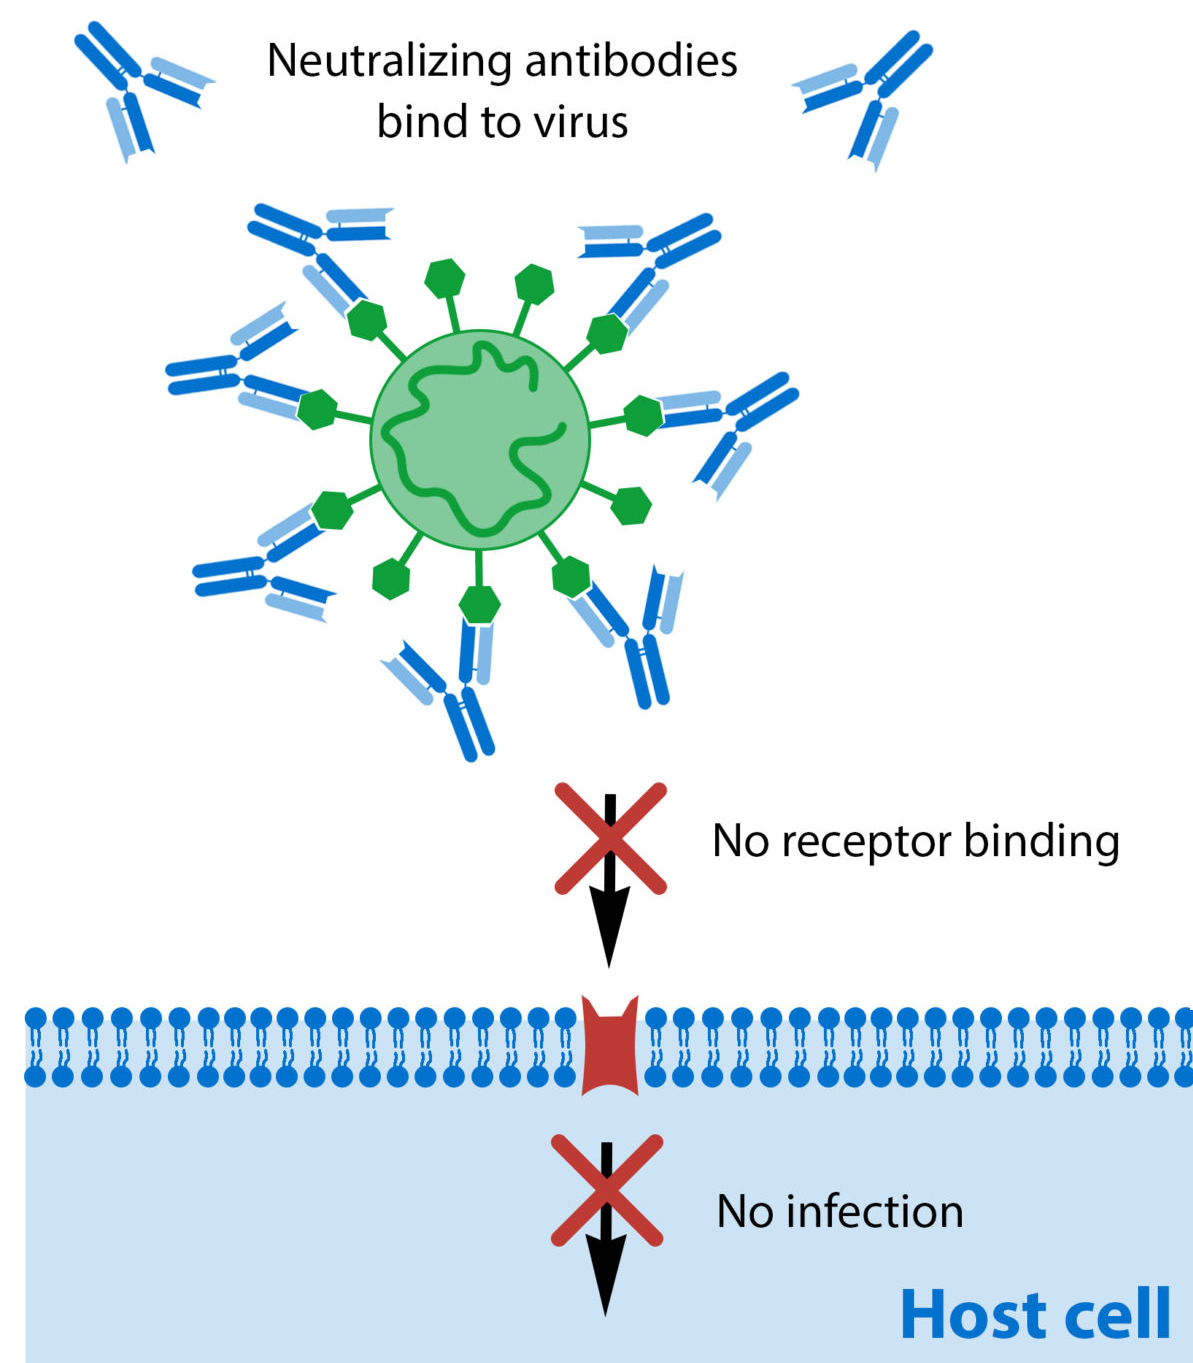
\includegraphics[width=\textwidth]{../Images/neutralization.png}   
        \caption{Neutralization of a pathogen by antibodies}
        \label{fig:neutralization}
    \end{minipage}
\end{figure}


\subsubsection{Phagocyte recruitment}

\subsubsection{Antibody Dependent Cell Cytotoxicity}

\subsubsection{Complement Dependent Cell Cytotoxicity}
